\documentclass[11pt]{article}
\usepackage[T1]{fontenc}
\usepackage{mathpazo}
\usepackage{amsmath,bm}
\usepackage{tikz}
\usetikzlibrary{arrows.meta,angles,quotes,calc,patterns}
\usepackage[paperwidth=170mm,paperheight=98mm,margin=4mm]{geometry}
\pagestyle{empty}
% the volume's palette, defined once and shared by every figure
\definecolor{ink}{HTML}{102A43}\definecolor{prim}{HTML}{1F6FEB}
\definecolor{acc}{HTML}{E85D04}\definecolor{crim}{HTML}{C1121F}
\definecolor{fore}{HTML}{2D6A4F}\definecolor{steel}{HTML}{486581}
\definecolor{blk}{HTML}{93C5C6}\definecolor{slope}{HTML}{E1E7EF}
\tikzset{
  force/.style={-{Stealth[length=2.6mm,width=1.9mm]},line width=1.15pt},
  body/.style={fill=blk,draw=steel,line width=0.6pt},
}
\begin{document}
\centering
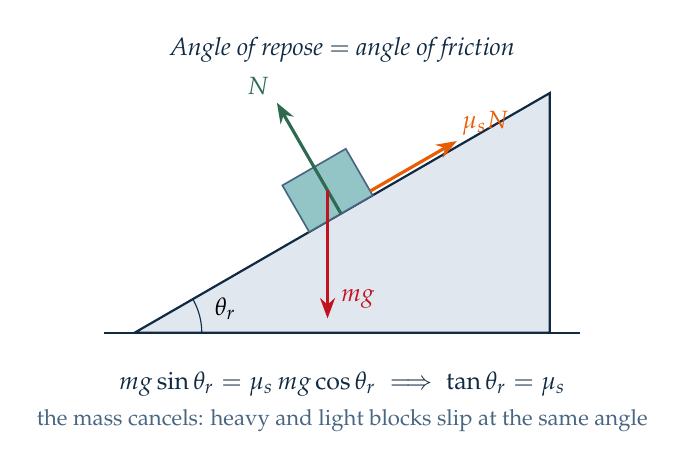
\begin{tikzpicture}[scale=1.55,font=\small]
  \def\th{30}
  % incline and ground
  \fill[slope,draw=ink,line width=0.8pt] (0,0) -- (3.4,0) -- (3.4,{3.4*tan(\th)}) -- cycle;
  \draw[ink,line width=0.8pt] (-0.25,0) -- (3.65,0);
  \coordinate (O) at (0,0); \coordinate (X) at (1,0); \coordinate (T) at (\th:1);
  \pic[draw=ink,angle radius=8.5mm,"$\theta_r$",angle eccentricity=1.4] {angle=X--O--T};
  % everything on the slope is placed in the slope's own frame
  \begin{scope}[shift={(\th:1.95)},rotate=\th]
    \draw[body] (-0.30,0) rectangle (0.30,0.44);
    \coordinate (C) at (0,0.22);         % centre of the block
    \coordinate (P) at (0,0);            % contact point
    \draw[force,fore] (P) -- (0,1.05) node[above left=-1pt] {$N$};
    \draw[force,acc]  (0.30,0.04) -- (1.12,0.04) node[above right=-2pt] {$\mu_s N$};
  \end{scope}
  \draw[force,crim] (C) -- ++(0,-1.05) node[right=1pt,pos=0.85] {$mg$};
  % the result, set in the same type as the text around it
  \node[ink] at (1.7,-0.42) {$mg\sin\theta_r=\mu_s\,mg\cos\theta_r\;\Longrightarrow\;\tan\theta_r=\mu_s$};
  \node[steel,font=\footnotesize] at (1.7,-0.72)
       {the mass cancels: heavy and light blocks slip at the same angle};
  \node[ink,font=\small\itshape] at (1.7,2.32) {Angle of repose $=$ angle of friction};
\end{tikzpicture}
\end{document}
